% Section 4 - Conflict Resolution and Anti-Entropy (Habib Hasanov)
% Figure: ../diagrams/antientropy_merkle.png (docs/diagrams/hasanov_diagrams.py)
% Citations: docs/references.bib
\section{Conflict Resolution and Anti-Entropy}\label{sec:antientropy}

Section~\ref{sec:consistency} showed that a write reaches all live replicas but is
acknowledged by only $W$ of them, so replicas can disagree after any failure. This section
explains how Cassandra decides \emph{which} version is correct (conflict resolution) and how
replicas that missed writes are brought back in line (anti-entropy). Experiment~4
(Section~\ref{sec:results-exp46}) isolates each mechanism.

\subsection{Last-write-wins per cell}

Every cell (one column of one row) carries a 64-bit write timestamp in microseconds. Our
driver assigns it on the client; \texttt{USING TIMESTAMP} overrides it, and without a client
value the coordinator assigns one. Whenever two versions of a cell meet---in a read, a hint,
read repair, repair streaming or compaction---the higher timestamp wins and the other version
is discarded~\cite{lakshman2010cassandra,cassdoc-dynamo}. Ties are broken deterministically: a
deletion beats a live value, and between two live values the byte-wise larger value wins,
so every replica independently reaches the same result without communicating. Because
reconciliation is per \emph{cell}, concurrent updates to different columns of one row both
survive; only updates to the same cell conflict.

Last-write-wins (LWW) makes physical clocks part of correctness. Timestamps are not
Lamport clocks~\cite{lamport1978time}: they do not capture causality, so a writer whose clock
runs ahead can win against a later write, and two causally ordered writes from different
clients can be reordered by skew. Production clusters therefore rely on NTP-synchronised
clients and nodes. In our testbed all containers share the host clock, which removes skew
from the measurements; Experiment~5 instead \emph{sets} timestamps with \texttt{USING
TIMESTAMP} to make the winner deterministic.

\paragraph{Why not vector clocks?}
Dynamo tracks causality with vector clocks~\cite{decandia2007dynamo,mattern1989vector}: when
two versions are concurrent, both are kept as \emph{siblings} and the application merges them
on its next read. Cassandra deliberately dropped this~\cite{lakshman2010cassandra}. LWW needs no
per-key version metadata that grows with the number of writers, no read-time merge logic in
every client, and no sibling explosion under contention, and it composes with the
log-structured storage engine: compaction can merge SSTables with a simple timestamp
comparison. The price is that \emph{concurrent} writes to the same cell are not detected:
one acknowledged write silently disappears. Experiment~5 shows this for a partition, and
the plain-\texttt{INSERT} race of Experiment~6 for concurrent clients; applications that cannot
tolerate it use lightweight transactions (Section~\ref{sec:consensus}) or counters.

\paragraph{Deletes are writes}
A \texttt{DELETE} writes a \emph{tombstone}, a timestamped marker that wins over older
values like any other cell. Tombstones are purged by compaction only after the table's
\texttt{gc\_grace\_seconds} (default 864\,000\,s, ten days)~\cite{cassdoc-tombstones}. If a
replica misses a delete and is not repaired before the tombstone is purged elsewhere, the
replica's old value is later streamed back as a ``zombie''---the deleted row reappears. Every
replica must therefore be repaired at least once per \texttt{gc\_grace\_seconds}, which is
the hard operational requirement behind the mechanisms below.

\subsection{Three repair mechanisms}

Fig.~\ref{fig:antientropy} and Table~\ref{tab:antientropy} compare the mechanisms. They differ in
what triggers them, what data they cover, and whether they can be relied on.

\begin{figure*}[t]\centering
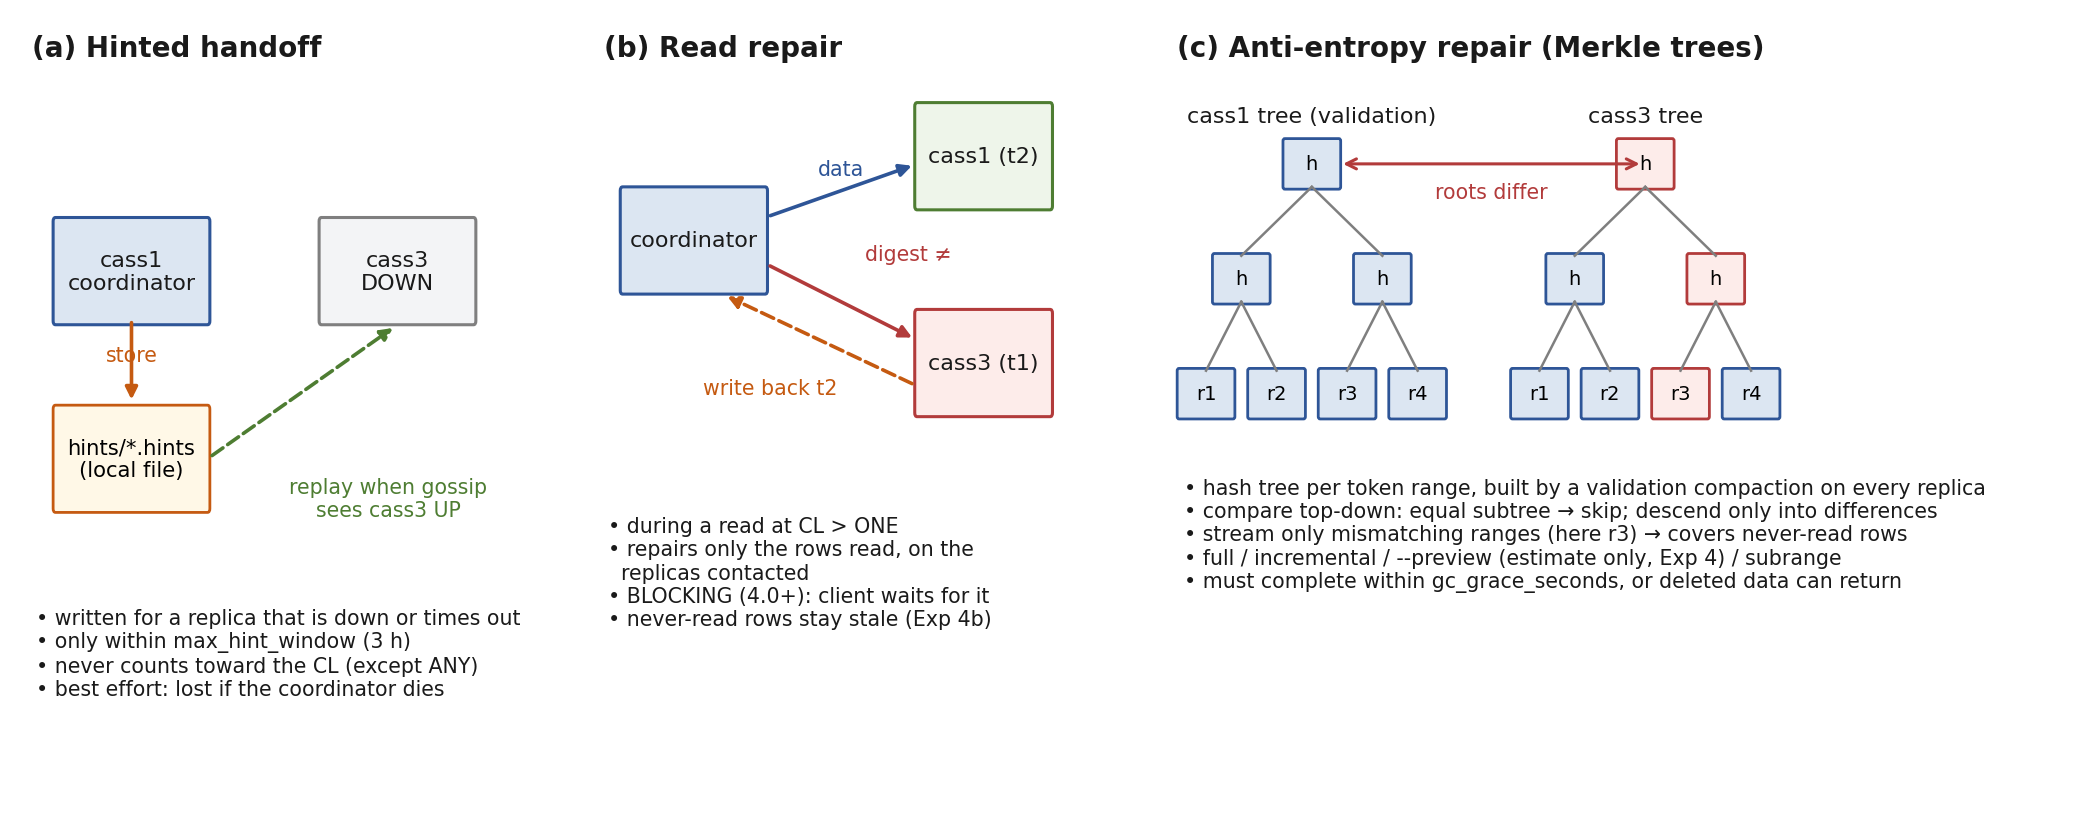
\includegraphics[width=0.92\textwidth]{antientropy_merkle.png}
\caption{Cassandra's three repair mechanisms: (a) hints written by the coordinator for a down
replica, (b) read repair on a digest mismatch, (c) Merkle-tree anti-entropy repair, which
narrows a mismatch to the token sub-ranges that must be streamed.}\label{fig:antientropy}
\end{figure*}

\paragraph{Hinted handoff}
When a coordinator sends a mutation to a replica that gossip reports as down, or that does
not acknowledge in time, it stores a \emph{hint} (target host ID plus mutation) in its local
\texttt{hints} directory; hints are buffered in memory and flushed to files periodically
(\texttt{hints\_flush\_period}, 10\,s). When gossip marks the target up again, the
coordinator streams the hints to it, throttled, and deletes each file once delivered.
Hints are written only while the target has been down for less than
\texttt{max\_hint\_window} (3\,h by default) and expire with the table's
\texttt{gc\_grace\_seconds}~\cite{cassdoc-hints}. They are a best-effort optimisation:
they never count towards the consistency level (except ANY,
Section~\ref{sec:consistency}), they are lost if the coordinator itself fails before
delivery, and a replica down longer than the window receives none.

\paragraph{Read repair}
During a read at a level that contacts more than one replica, the coordinator compares a
data response with digests; on a mismatch it fetches full data, reconciles by LWW and
writes the winning cells back to the stale replicas it contacted. Since 4.0 this is
\emph{blocking}: the client is answered only after the repair writes are acknowledged, which
makes successive quorum reads monotonic (Section~\ref{sec:consistency}). The
probabilistic background variant (\texttt{read\_repair\_chance}) was removed in 4.0 and
replaced by the per-table \texttt{read\_repair} option (\texttt{BLOCKING} or
\texttt{NONE})~\cite{cassdoc-readrepair}. Read repair is \emph{opportunistic}: it repairs only
rows that are read, at a level above ONE, on the replicas that the read touched. Rows that are
never read stay divergent, which Experiment~4b demonstrates with a control sample.

\paragraph{Anti-entropy repair}
\texttt{nodetool repair} compares whole token ranges. Each replica of a range runs a
\emph{validation compaction} that hashes its data into a Merkle tree~\cite{merkle1987}:
leaves cover contiguous token sub-ranges and every inner node hashes its children. The
initiator compares the trees top-down; equal subtrees are skipped, so only sub-ranges whose
leaf hashes differ are streamed between replicas, and LWW reconciles the streamed data on
arrival. This is the only mechanism that covers \emph{all} data, including never-read rows
and missed deletes. \emph{Full} repair rebuilds trees over all SSTables; \emph{incremental}
repair (the default command since 2.2, made reliable in 4.0) validates only SSTables not yet
marked repaired and then anti-compacts them into a repaired set; \texttt{-pr} limits a node
to its primary ranges and \texttt{-st}/\texttt{-et} to a subrange~\cite{cassdoc-repair}.
\texttt{--preview} builds and compares the trees but only reports the streaming that would
occur~\cite{cass13257}; Experiment~4 uses it as a non-invasive divergence detector before
and after each mechanism. Repair costs disk and network I/O proportional to the data, so in
5.0 it is scheduled by the operator (or an external tool). Cassandra 6.0 adds a built-in
scheduler (CEP-37~\cite{cep37,cassdoc-autorepair}); it is disabled by default and was not
available in our 5.0.8 cluster.

\begin{table}[t]\centering\footnotesize
\caption{Repair mechanisms in Cassandra 5.0.}\label{tab:antientropy}
\begin{tabular}{@{}p{0.2\columnwidth}p{0.22\columnwidth}p{0.22\columnwidth}p{0.24\columnwidth}@{}}\hline
 & Hinted handoff & Read repair & Anti-entropy repair \\ \hline
Trigger & write to a down / slow replica & digest mismatch in a read at CL $>$ ONE & operator / scheduler \\
Scope & writes missed during $\le$ 3\,h & rows read, replicas contacted & all data of the repaired ranges \\
Timing & on recovery (gossip UP) & inline, blocks the read & offline batch \\
Guarantee & best effort & read rows monotonic & complete if it finishes \\
Cost & hint storage on coordinator & extra read latency & validation compaction + streaming \\ \hline
\end{tabular}
\end{table}

\paragraph{How they combine}
The mechanisms are layered by cost. Hints repair short outages almost for free; read repair
fixes hot data on the critical path; anti-entropy is the safety net that bounds divergence in
time and makes deletes durable. None of them changes what a client can observe at
$R + W > N$---that guarantee comes from quorum intersection
(Section~\ref{sec:consistency}); they shorten the window in which lower levels can return
stale data and keep the replicas within the \texttt{gc\_grace\_seconds} contract.
